\documentclass[a4paper, 12pt]{report}
\usepackage[utf8]{inputenc}
\usepackage[french]{babel}
\usepackage[T1]{fontenc} % permettent d'utiliser tous les caractères du clavier.
\usepackage{inputenc} % permettent d'utiliser tous les caractères du clavier.
\usepackage[top=2.0cm, bottom=2.0cm, left=2.0cm, right=2.0cm]{geometry} %marges des pages
\usepackage{color}
\usepackage{fancyhdr} %apparence globale
\usepackage {hyperref} %table des matières avec liens ds le dossier.
\usepackage{graphicx} %image
\usepackage{setspace}


\definecolor {colortitre1}{rgb}{0.2,0.4,0.2}
\definecolor {colortitre2}{rgb}{0.2,0.5,0.2}
\definecolor {colortitre3}{rgb}{0.2,0.6,0.1}
\pagestyle{plain}

\title{Projet \\POO - Réseau \\ Aquarium}
\author {FALTREPT Bérénice \\ ESPIAUT Marc-Alexandre}
\date{année 2014/2015}

\begin{document}
	\begin{spacing}{1.3}
\maketitle%sert a afficher le title dans le document, sinon serait des méta données.
\tableofcontents
\newpage
\textcolor{colortitre1}{\section*{Présentation}}
\addcontentsline{toc}{section}{Présentation}

Notre projet est centré sur un aquarium distribué. L'objectif étant que les items mobiles de l'aquarium soient dépendant d'un aquarium créateur mais visibles sur les clients connectés au serveur.

Le code du projet est récupérable via git grace à la commande suivante\\
\texttt{git clone https://github.com/bfaltrep/Reseau.git}

\textcolor{colortitre1}{\subsection*{Travail effectué}}
\addcontentsline{toc}{subsection}{Travail effectué} 	
	
Nous avons mis en place un exécutable pouvant être soit serveur soit client en fonction de la demande de l'utilisateur via les paramètres. Dans les deux cas, l'utilisateur a accès à un aquarium disposant de ses classes locales capable de se reproduire et les deux classes fournies nativement ont la fonctionnalité \textit{piscivore} : une classe est capable de manger l'autre.
	
Une fois le contact établi entre le serveur et un client, les classes et les items mobiles créés dans le client, puis ceux déjà existants dans le serveur, sont transmit pour être présents dans les divers aquariums.
	
\textcolor{colortitre2}{\subsection*{Avantages}}
\addcontentsline{toc}{subsection}{Avantages}

Nous avons actuellement un aquarium animé dont une partie des items mobiles proviennent effectivement d'autres poste. Certaines fonctionnalités permettent d'apporter du changement dans la "faune" de l'aquarium pour lui apporter quelques intérêts.
	
\textcolor{colortitre2}{\subsection*{Bugs connus}}
\addcontentsline{toc}{subsection}{Bugs connus}

Les poissons se reproduisent beaucoup trop vite. Cela aurait pu être corrigé avec du temps supplémentaire. Cela est du au fait que le programme ne prends pas en compte que deux poissons se sont déjà reproduits une fois. Une correction simple aurait été de limiter la taille des listes d'éléments.
	
Nos transmissions entre serveur et clients sont imparfaites : actuellement les objets transmit sont limités en nombre. La transmission des positions est correcte mais leur application ne se fait pas.
	
Les poissons arrivés n'ont pas de cible précise. Ce n'était pas nécessaire sachant que leurs positions sont supposés être mises à jour régulièrement depuis le client qui définit leurs caractéristiques, ils ont tendance à quitter l'aquarium par la droite.
	
	
\textcolor{colortitre1}{\subsection*{Les Modules}}
\addcontentsline{toc}{subsection}{Les Modules}

%Diagramme des classes
Le nombre de classes indispensables à ce projet nous a été fourni dans la base du code du projet.

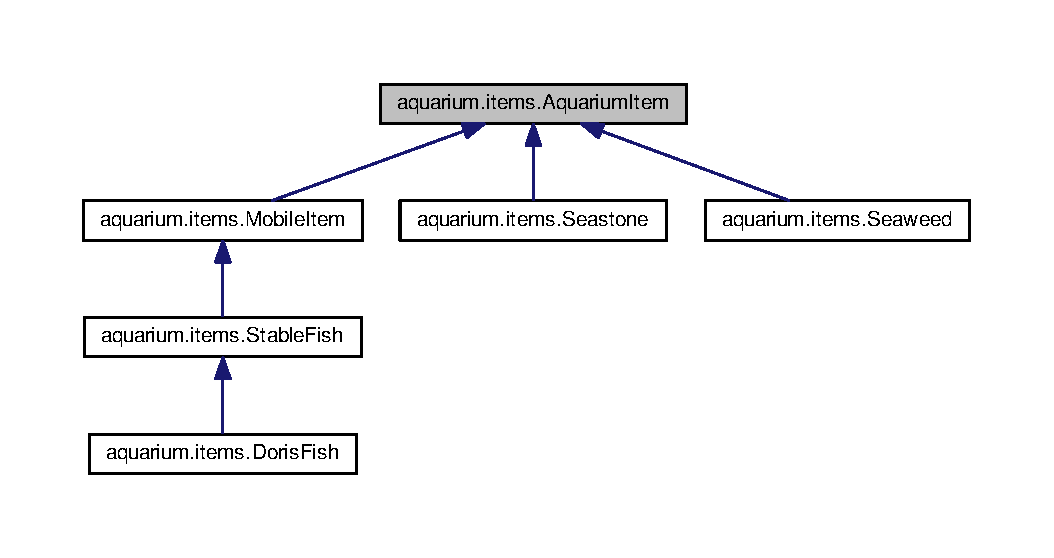
\includegraphics[scale=1]{graphique.pdf}

\newpage

\textcolor{colortitre2}{\section*{Les classes statiques}}
\addcontentsline{toc}{section}{Les classes statiques} 
	
\textcolor{colortitre3}{\subsection*{Main}}
\addcontentsline{toc}{subsection}{Main} 
		
Cette classe sert, comme son nom l'indique, au lancement de l'exécution du programme. elle permet notamment de tenir compte des arguments donnés par l'utilisateur pour lancer soit un serveur, soit un thread client.
		
\textcolor{colortitre3}{\subsection*{Constante}}
\addcontentsline{toc}{subsection}{Constante} 
Cette classe est une énumération des commandes acceptées par notre protocole. Elle permet d'assurer la conformité des commandes qui seront passées, mais surtout de rendre le code du protocole plus lisible.

\textcolor{colortitre3}{\subsection*{Protocole1}}
\addcontentsline{toc}{subsection}{Protocole1}
		
Il s'agit de l'implémentation de notre protocole. Il formate les informations pour envoyer les données et récupère les informations depuis les String reçus. Suivant le protocole choisit sur le framapad commun, nous avons choisi un transfert des informations par String où la séparation entre les commandes est faite par le symbole "\#" et la séparation des données au sein d'une commande se fait par "!".

\newpage

\textcolor{colortitre2}{\section*{Les classes instanciables}} \addcontentsline{toc}{section}{Les classes instanciables}

\textcolor{colortitre3}{\subsection*{ServerThread}}
\addcontentsline{toc}{subsection}{ServerThread}

Le ServerThread est la classe instancié si l'utilisateur lance un serveur via le main.

Elle créée les variables nécessaires au contact avec les clients mais aussi à la gestion de l'aquarium initial du serveur.

Pour s'assurer que le nombre de clients ne posera pas de problèmes durant l'exécution, nous utilisons la classe \textit{ScheduledExecutorService} qui va créer 10 Threads. Ces Threads traiteront les envois et réceptions des sockets des clients, quel que soit leur nombre.
	
\textcolor{colortitre3}{\subsection*{Client}}
\addcontentsline{toc}{subsection}{Client}

La classe Client est instancié lorsque l'utilisateur demande à se connecter en tant que client à un serveur. C'est une classe qui étend la classe Thread et qui va, elle aussi, utiliser une instance de \textit{ScheduledExecutorService}, mais cette fois avec seulement trois Threads car il n'a qu'un seul contact à traiter.
		
\textcolor{colortitre3}{\subsection*{ClassesMobiles}}
\addcontentsline{toc}{subsection}{ClassesMobiles}
		
Cette classe est utilisée pour stocker les différent types, donc classes, d'items mobiles utilisés dans l'aquarium. Une liste de ClassesMobiles se trouve dans l'aquarium. Elle contient toutes les classes actuellement présentes dans l'aquarium.

Cette classe a été initialement conçue pour permettre de transférer les images des différentes classes et les stocker.

Ainsi nous aurions pu ne les envoyer qu'une seule fois et faire une économie de bande passante.

Malheureusement, nous n'avons pas eu le temps d'implémenter le transfert d'images, elle a donc actuellement un usage moins essentiel.

\textcolor{colortitre3}{\subsection*{Aquarium}}
\addcontentsline{toc}{subsection}{Aquarium}
		
	La classe aquarium nous a été fournie, mais de nombreuses modifications sont intervenues et ses fonctionnalités ont changées.
	Tout les accès aux variables de la classe se font via des accesseurs qui limitent les risques de mauvaises manipulation par le/les protocole(s) qui peuvent être utilisés.
	
L'organisation des items a été changée, il y a à présent trois listes.
\begin{itemize}
\item Une reprenant les items initiés dans cet aquarium, mobiles ou non.
\item Une seconde contenant une représentation simplifiée des instances mobiles créées dans un aquarium en contact avec celui-ci.
\item La dernière contient à chaque instant la liste des classes d'éléments mobiles actuellement présentes dans l'aquarium.
\end{itemize}
	
Ceci pour permettre d'avoir un premier tri des items et de ne pas avoir à parcourir l'ensemble d'une liste contenant des items créés localement et d'origines éloignés pour accéder à un item en particulier.

\newpage

\textcolor{colortitre1}{\section*{Conclusion}}
\addcontentsline{toc}{section}{Conclusion}

Le sujet, à la fois simple et visuel, est intéressant pour un tout premier projet en réseau.

Pour des débutants, il est satisfaisant de voir les effets concrets de nos modifications sur le code du projet. Mais surtout, faire de la programmation objet était un souhait pour l'un d'entre nous. ce fut donc intéressant.

Ceci dit, nous regrettons de ne pas avoir aboutit nos plans, qui se sont avérés trop grands. Nous avions prévus de faire passer les images des poissons entre les différents protagonistes, mais cela n'a pas été possible à cause d'une organisation limitée.

Plus gênant, des fonctionnalités plus basiques que nous avons commencés à implémentées n'ont pas encore l'action souhaitée de façon optimum : surpopulation, non transfert de tout les poissons, problème de mise à jour des positions.

Ceci dit, cela reste une bonne expérience en réseau comme pour la programmation orienté objet et nous espérons continuer à nous améliorer par la suite.

\end{spacing}
\end{document}





